\chapter{Introduction}
\label{chap:intro}

Data sketches, or \emph{sketches} for short, are indispensable tools for performing analytics on high-rate, high-volume incoming data streams~\cite{KDD_tutorial}. A case study made by Yahoo has shown the impact of sketches on data analytics. Flurry~\cite{flurry} is a mobile application real-time analytics platform, acquired by Yahoo in 2014. Using data sketches architecture in Flurry reduced the overall cost of the system considerably. Sketches led to a reduction in data processing times from days or hours to minutes and even seconds~\cite{flurry_case}.


Sketches typically estimate some function of a large data stream, for example, the frequency of certain items, or how many unique items have appeared. Sketches are quantitative objects that support update and query operations, where the return value of a query is from a totally ordered set. 


Sketches are designed for stream settings in which each data item is only processed once. A sketch data structure is essentially a succinct (sublinear) summary of a data stream that approximates a specific query (unique element count, quantile values, etc.). Since summaries have a much smaller size, they typically answer queries approximately, and there is a trade-off between the size of the summary and the approximation error. Some sketches can be deterministic, although most sketches are probabilistic in their behavior and take advantage of various randomization techniques. Typical sketches are \emph{probably approximately correct (PAC)}, estimating some aggregate quantity with an error of at most $\epsilon$ with a probability of at least $1-\delta$ for some parameters $\epsilon$ and $\delta$~\cite{mergeables_summaries, Cormode2011SketchTechniques, Rinberg_2020_fast_sketches, Zhao2021KLLPlus}.


Some sketches have a well-known mergeability property~\cite{mergeables_summaries}, which enables computing a sketch over a stream by merging sketches over sub-streams and merging them into a single sketch whose error is no greater than if it had processed the entire stream. The ever-increasing rates of incoming data create a strong demand for parallel stream processing~\cite{Cormode_2011_disributed_monitoring, Heule_2013_cardinality_est}. Previous works have exploited the mergeability property for distributed stream processing, devising solutions with a sequential bottleneck at the merge phase.


With the rise of big data, a fundamental task in data management and data analysis is to describe the distribution of the data. This is used in applications such as exploratory data analysis~\cite{vartak2015seedb}, operation monitoring~\cite{abraham2013scuba}, and more. If the distribution is known a priori, such as a normal or zipifian distribution, it can be described by the parameters of the distribution. This is rarely the case in practice, which calls for describing the distribution nonparametrically. Quantiles are the most commonly used nonparametric representation for data distribution. In particular, a technique such as quantile approximation, a nonparametric representation, is widely used to characterize data distributions~\cite{WangLuoYiCormode2013, Zhao2021KLLPlus}.


This problem has attracted a lot of prior studies, from both the algorithms and the database communities~\cite{MunroPeterson1980, MankuRajagoplanLindsay1998, HungTing2010Omega, mergeables_summaries, DataSketches}. Quantiles are of interest to both database implementers and users: for instance, they are a fundamental tool for query optimization~\cite{MankuRajagoplanLindsay1998}, splitting of data in parallel database systems~\cite{PoosalaIoannidis1996EstimationOfQueryDistiributionAndAppInParallel, Cormode_2011_disributed_monitoring, Heule_2013_cardinality_est}, and statistical data analysis~\cite{Indyk2004GeometricProblems, Cranor2003Gigascope}. In the past years, quantile estimation has received particular attention in the data streaming model, i.e., the data elements arrived one by one in a streaming fashion, and the algorithm has limited memory to work with~\cite{MunroPeterson1980, MankuRajagoplanLindsay1998, MankuRajagoplanLindsay1999, Greenwald2001_online_computation, Gilbert2002SummarizeUniverse, Shrivastava2004Qdigest, Cormode2005CountMinSketch, HungTing2010Omega, mergeables_summaries, KarninKevinLiberty2016, Zhao2021KLLPlus}. 


The quantiles correspond to the \emph{cumulative distribution function (CDF)}, which yields the \emph{probability density function (PDF)}. They are a generalization of the median. Given $A$, a multi-set of $n$ elements is drawn from a totally ordered universe, the $\phi$-quantile of $A$, for some  $0 \leq \phi \leq 1$, is the element whose rank is $\lfloor \phi n \rfloor $ in $A$, where the rank of an element $x$ is the number of elements in $A$ smaller than $x$. Note, given enough space, the quantiles can be easily found by sorting the set $A$.


Yet, when the algorithm's memory is limited and significantly smaller than the size of the data set, it is not possible to compute the quantile precisely. This was formalized in a 1980 paper by Munro and Peterson~\cite{MunroPeterson1980}. They have shown that computing the median with $p$ passes over $A$ has to use $\Omega(n^{-p})$ space. Thus, computing the true median will require memory linear in the size of the set. An alternate and more practical approach to the problem is to approximate the quantiles, represented as $\epsilon$ approximation $\phi$-quantile: For an error parameter $0<\epsilon<1$, the $\epsilon$-approximate $\phi$-quantile is any element between $(\phi-\epsilon)n$ and $(\phi+\epsilon)n$.


The Quantiles sketch family captures this task~\cite{masson2019ddsketch, mergeables_summaries, gan2018moment, cormode2021relative}. The Quantiles sketch represents the quantiles distribution in a stream of $n$ elements, such that for any $0 \leq \phi \leq 1$, a query for quantile $\phi$ returns an estimate of the $\lfloor n\phi \rfloor ^{\text{th}}$ largest element. Due to the importance of quantiles approximation, Quantiles sketches are a part of many analytics platforms, e.g., Druid~\cite{druid-quantiles}, Hillview~\cite{budiu2019hillview}, Presto~\cite{presto}, and Spark~\cite{spark}.


The deterministic $\epsilon$-approximation $\phi$-quantile algorithms take as input a quantile query $\phi$ and a precision value $\epsilon$ and output an element $x$ such that the quantile of $x$ is in the range $[\phi-\epsilon, \phi+\epsilon]$. An alternative approach proposes a family of randomized algorithms where the output answer $x$ is within the $[\phi-\epsilon, \phi+\epsilon]$ range with a high probability~\cite{MankuRajagoplanLindsay1999, KarninKevinLiberty2016}. These algorithms provide guarantees by bounding the failure probability to at most $\delta$ such that the user has $1-\delta$ confidence that the sketch’s output is $\epsilon$-approximation.


The first deterministic streaming algorithm for quantiles was proposed by Manku, Rajagoplan, and Lindsay~\cite{MankuRajagoplanLindsay1998}, building on the prior work by Munro and Paterson~\cite{MunroPeterson1980}. This algorithm has space complexity $O(\frac{1}{\epsilon}\log^2(\epsilon n))$, meaning that using memory that grows poly-logarithmically in the stream size and inversely with the accuracy parameter $\epsilon$, the quantiles can be estimated with precision $\epsilon n$. We refer to this algorithm as MRL. This result has since been improved by two groups: 
In 2001, Greenwald and Khanna~\cite{Greenwald2001_online_computation} designed a deterministic comparison-based algorithm (referred to as the GK algorithm) and showed that it uses $O(\frac{1}{\epsilon}\log(\epsilon n))$ space in the worst case. Hung and Ting~\cite{HungTing2010Omega} showed an $\Omega (\frac{1}{\epsilon}log(\epsilon n))$ lower bound for these deterministic algorithms. In this category, the GK algorithm is generally considered to be the best but it is not known to be mergeable.
In 2004, Shrivastava et al.~\cite{Shrivastava2004Qdigest} designed a deterministic, fixed-universe algorithm, called Q-digest, that uses $O(\frac{1}{\epsilon}\log(u))$ space, where $[u]$ is a fixed finite universe from which the elements are drawn, meaning that the universe has to be known. This algorithm was designed for quantile computation in sensor networks and is a mergeable summary~\cite{mergeables_summaries}. %Note that the $\log(u)$ and $\log(\epsilon n)$ terms are not comparable in theory.


In recent years, the community has turned to improving randomized approaches. Manku et al.~\cite{MankuRajagoplanLindsay1999} present an algorithm that does not need advance knowledge of $n$, and showed its space requirements to be $O (\frac{1}{\epsilon}log^{2}(\frac{1}{\epsilon}))$. However, they must give up the deterministic guarantee on accuracy. Instead, they provide only a probabilistic guarantee that the quantile estimates are within the desired precision.
Agarwal et al.~\cite{mergeables_summaries} presented a mergeable algorithm with a space complexity of $O (\frac{1}{\epsilon}log^{1.5}(\frac{1}{\epsilon}))$. Karnin, Lang, and Liberty (KLL)~\cite{KarninKevinLiberty2016} presented the KLL sketch, a randomized algorithm based on techniques from GK and the Quantiles sketch proposed in~\cite{mergeables_summaries}. KLL is an asymptotically optimal non-mergeable sketch that solves the problem using $O (\frac{1}{\epsilon}\log \log(\frac{1}{\delta}))$ space. Karnin et al. also presented a mergeable KLL sketch with $O (\frac{1}{\epsilon}\log^2 \log(\frac{1}{\delta}))$ space bounds.



\begin{table}[h]
\caption{Comparison between different Quantiles sketches.}
\label{table:compare-quantiles}
\centering
\renewcommand{\arraystretch}{1.3}
  \begin{tabular}{  l  l  c  c } \toprule
    Algorithm                                       & \multicolumn{1}{c}{Space}                                    & Randomization & Mergeable \\ \midrule
    GK~\cite{Greenwald2001_online_computation}      & $O(\frac{1}{\epsilon}\log(\epsilon n))$   & Deterministic &    No    \\ \hline
    Q-digest~\cite{Shrivastava2004Qdigest}          & $O(\frac{1}{\epsilon}\log(u))$            & Deterministic &    Yes    \\ \hline
    MRL~\cite{MankuRajagoplanLindsay1998}           & $O(\frac{1}{\epsilon}\log^2(\epsilon n))$   & Deterministic &    Yes    \\ \hline
    MRL99~\cite{MankuRajagoplanLindsay1999}         & $O(\frac{1}{\epsilon}\log^2(\frac{1}{\epsilon})$   & Randomized &    Yes    \\ \hline
    KLL~\cite{KarninKevinLiberty2016}               & $O(\frac{1}{\epsilon}\log\log(\frac{1}{\delta})$   & Randomized &    No    \\ \hline
    Mergeable KLL~\cite{KarninKevinLiberty2016}     & $O(\frac{1}{\epsilon}\log^2\log(\frac{1}{\delta})$   & Randomized &    Yes    \\ \hline
    Quantiles Sketch~\cite{mergeables_summaries}    & $O(\frac{1}{\epsilon}\log^{1.5}(\frac{1}{\epsilon})$   & Randomized &    Yes    \\
    % \hline
    \bottomrule
  \end{tabular}
\end{table}


% %Sketches are designed for \emph{stream} settings, in which each element is processed once. 
% Like other sketches, existing Quantiles sketches are of sublinear-size and their estimates are \emph{\gls{PAC}}, providing an approximation within some error $\epsilon n$ with a failure probability bounded by some parameter $\delta$. 
% The sequential solution proposed by Agarwal et al.~\cite{mergeables_summaries} is used by Apache DataSketches~\cite{DataSketches}, and our concurrent sketch is based on. This Quantiles sketch is of sublinear-size and his estimates are \emph{\gls{PAC}}, providing an approximation within some error $\epsilon n$ with a failure probability bounded by some parameter $\delta$.
The mergeable Quantiles sketch proposed by Agarwal et al.~\cite{mergeables_summaries} is very popular and forms a basis for many works that followed~\cite{KarninKevinLiberty2016, WangLuoYiCormode2013}. The sequential solution proposed in~\cite{mergeables_summaries} is used by Apache DataSketches~\cite{DataSketches}, and our concurrent sketch is based on it. This Quantiles sketch is of sublinear-size and his estimates are \emph{\gls{PAC}}, providing an approximation within some error $\epsilon n$ with a failure probability bounded by some parameter $\delta$.


In the context of sequential processing, the classic literature on sketches has focused on inducing a small error while using a small memory footprint: The sketch is built by a single thread, and queries are served only after the sketch construction is complete. Only recently, we begin to see works leveraging parallel architectures to achieve a higher ingestion throughput while also enabling queries concurrently with updates~\cite{Rinberg_2020_fast_sketches, stylianopoulos2020delegation}. 
Of these, the only solution suitable for quantiles that we are aware of is the \acrfull{FCDS} framework proposed by Rinberg et al.~\cite{Rinberg_2020_fast_sketches}. FCDS presents a generic algorithm for parallelizing data sketches efficiently and allowing them to be queried in real time. In general, FCDS is fast and achieves high scalability while keeping the estimation error small. The architecture of FCDS is based on local buffering of updates and constantly propagating results to a shared memory. Update threads ingest updates to local buffers. When a local buffer is full, its content is propagated to a shared global sketch. A single thread, called the propagator, propagates elements from all local buffers to the global sketch. Query threads access the global sketch.
In the FCDS-based Quantile sketch, the local buffers are sequential Quantiles sketches. Each update thread updates its local sketch and when it is full, signals the propagator. As mentioned above, the propagation of the local sketches into the global sketch is made only by the propagator while other update threads may be idle. When FCDS is used for quantiles, the process of propagation includes a heavy merge-sort, therefore, by using a single propagator, a sequential bottleneck is formed. Consequently, large local buffers are required to offset the heavy sorting and keep the working threads busy during propagations (resulting in a high relaxation and low query freshness). The scalability of FCDS-based Quantiles sketches is thus limited unless large buffers are used, causing query freshness to be heavily compromised (as we show below). Our goal is to provide a scalable concurrent Quantiles sketch that retains a small error bound with reasonable query freshness.


In Chapter~\ref{chap:background} we formally define the system model and the problem and also overview a popular sequential solution proposed by Agarwal et al.~\cite{mergeables_summaries}, which is used by Apache DataSketches~\cite{DataSketches}, on which our concurrent sketch is based.


In Chapter~\ref{chap:quancurrent}, we present \mysketch, our highly scalable concurrent Quantiles sketch.
Like FCDS, \mysketch relies on local buffering of stream elements, which are then propagated in bulk to a shared sketch.
But \mysketch improves on FCDS by eliminating the latter's sequential propagation bottleneck, which mostly stems from the need to sort large buffers.

In \mysketch, sorting occurs at three levels -- a small thread-local buffer, an intermediate \acrshort{NUMA}-node-local buffer called $\mathit{Gather\&Sort}$, and the shared sketch.
Moreover, the shared sketch itself is organized in multiple levels, which may be propagated (and sorted) concurrently by multiple threads.

To allow queries to scale as well, \mysketch serves them from a cached snapshot of the shared sketch.
This architecture is illustrated in Figure~\ref{fig:quancurrentDS}.
The query freshness depends on the sizes of local and NUMA-local buffers as well as the frequency of caching queries.
We show that using this architecture, high throughput can be achieved with much smaller buffers (hence much better freshness) than in FCDS.


% In Section~\ref{sec:background} we formally define the problem and overview a sequential solution proposed in~\cite{mergeables_summaries} and used by Apache DataSketches~\cite{DataSketches}. 
% In Section~\ref{sec:Quancurrent} we present Quancurrent, a thread-friendly version of the Quantiles sketch proposed in~\cite{mergeables_summaries}.
% We achieve high multi-threaded throughput by buffering data and propagating it to the shared sketch in bulk.
% As depicted in Figure~\ref{fig:quancurrentDS}, we use both local and shared buffers alongside a shared sketch data structure. The local buffers are non-atomically moved to the shared buffer, and the shared buffer is periodically propagated to the queryable state. The state is updated using CAS-based primitives, in a manner that ensures lock-freedom. At its base, the sequential Quantiles sketch uses a sort operation. \mysketch utilizes this mixture of local and shared buffers to mask these sorts and to allow more concurrency. 

\begin{figure}[htp]
    \centering
    \hspace{70pt}
        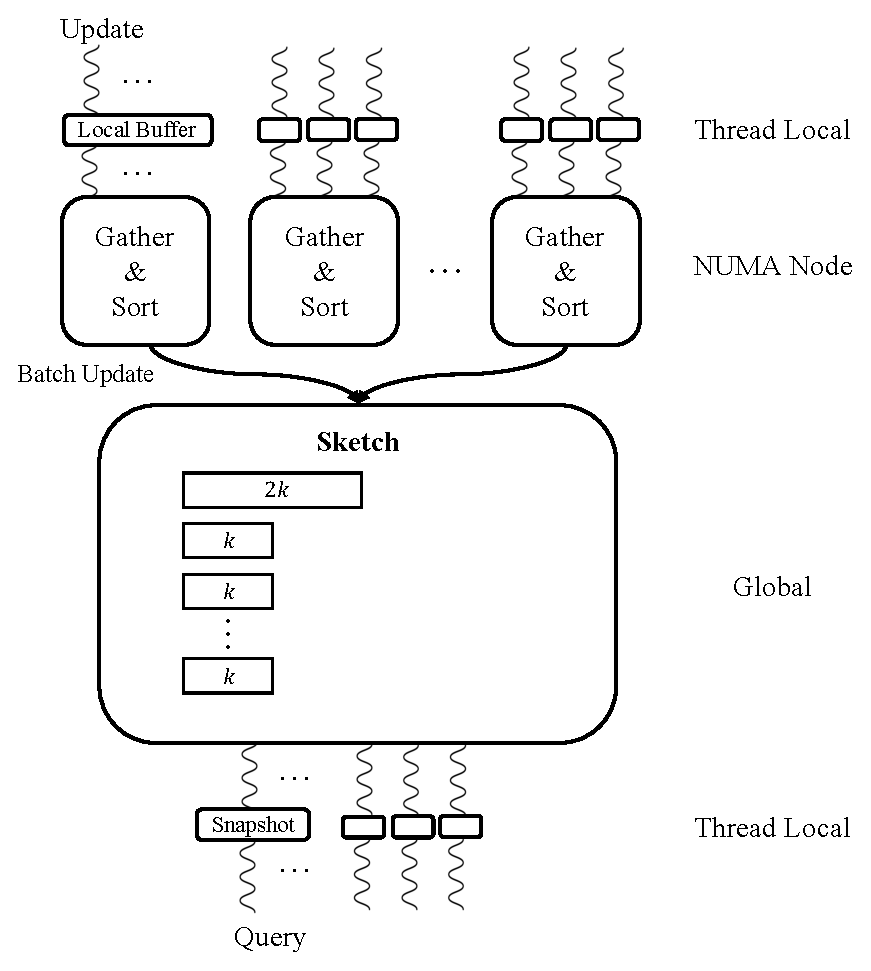
\includegraphics[width=0.8\linewidth,trim={0cm 0cm 0cm 0.1cm},clip]{graphics/algorithm/architecture.pdf}
    \caption{\mysketch's architecture.}
    \label{fig:quancurrentDS}
\end{figure}

% For scalability purposes, queries are served from a cached snapshot of the sketch. How up-to-date the query estimation depends on the sizes of the local and shared buffers and on the freshness of the cached snapshot, both of which are controlled by parameters.

To lower synchronization overhead, we allow buffered elements to be sporadically overwritten by others without being propagated, and others to be duplicated, i.e., propagated more than once. These occurrences, which we call \emph{holes}, alter the stream ingested by the data structure. 
Yet, in Chapter~\ref{chap:analysis} we show that for a sufficiently large local buffer, the expected number of holes is less than $1$ and because they are random, they do not change the sampled distribution.


Figure~\ref{fig:intro-query-accuracy} presents quantiles estimated by \mysketch on a stream of normally distributed random values compared to an exact, brute-force computation of the quantiles, and shows that the estimation is very accurate.

\begin{figure}[htp]
    \centering
    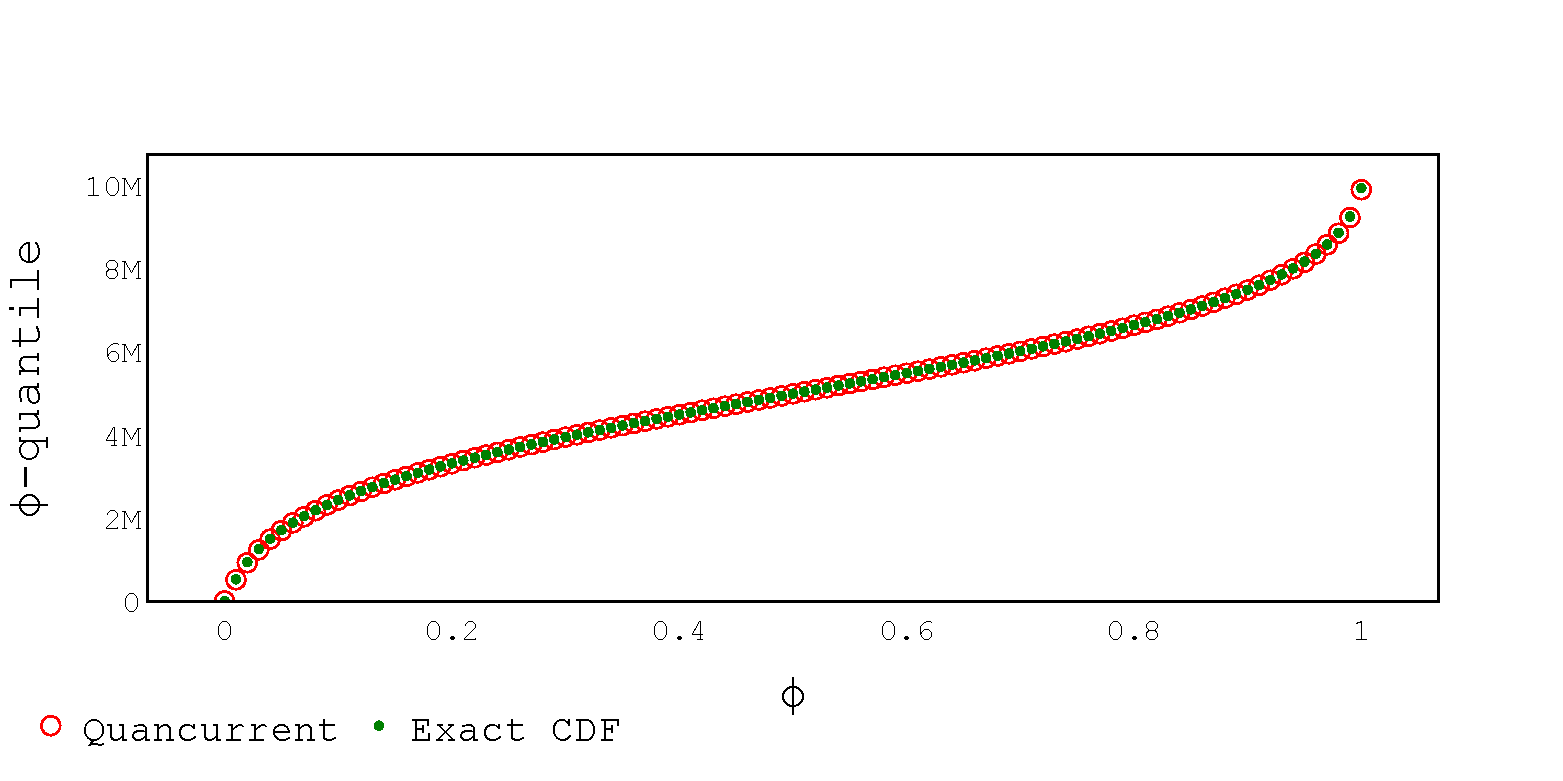
\includegraphics[width=\linewidth,trim={0cm 0.3cm 0cm 1.5cm},clip]
    {graphics/graphs/accuracy/Oracle_Quancurrent_blocking_numa_cdf_normal_k1024_b16_keys10M_runs1_uT32_qT1_snapshot1_17-09-2022_07-00-49.pdf}
    \caption{\mysketch's $\phi$-quantiles vs. exact quantiles (normal distribution, $k=1024$, $32$ update threads, $10M$ elements).}
    \label{fig:intro-query-accuracy}
\end{figure}


In Chapter~\ref{chap:eval} we empirically evaluate \mysketch. We show an update speedup of $12$x and a query speedup of $30$x over the sequential sketch, both with linear speedup. We compare \mysketch to FCDS, which is state-of-the-art in concurrent sketches. We show that for FCDS to achieve similar performance it requires an order of magnitude larger buffers than \mysketch, reducing query freshness tenfold.

In Chapter~\ref{chap:correctness} we present a formal correctness proof. Finally, Chapter~\ref{chap:conclusion} concludes our work and presents some open questions for future research. 


\section{Summary of Contributions} 
We present \mysketch, a scalable Quantiles sketch that retains a small error bound with reasonable query freshness. The main technical challenges we address are:
\begin{enumerate}
  \item High scalability. \mysketch's throughput increases linearly with the number of available threads. High throughput can be achieved with much smaller buffers (hence better query freshness).
  \item Accurate estimates (small error bound, fresh query). \mysketch allows queries to occur concurrently with updates and achieves better query freshness than existing scalable solutions. 
  \item Eliminating sequential propagation bottleneck. \mysketch allows more concurrency than previous solutions by utilizing multiple buffers and allowing multiple threads to concurrently engage in merge-sorts, which are a sequential bottleneck in previous solutions. 
  \item Minimizing synchronization. We leverage the fact that sketches are approximate to begin with to dramatically reduce the synchronization overhead.
  \item Correctness semantics with guaranteed error bounds. \mysketch query's snapshot is strongly linearizable with respect to an r-relaxed sequential Quantiles sketch with \(r=4kS + (N-S)b\).
\end{enumerate}


